\chapter{Геймификация в играх}
Прежде чем говорить о самой теме, об использовании геолокации в Android, имеет смысл рассказать о жанре игры, которая разработана в рамках данной работы.

Как и в случае с большинством игр, занятия физической активностью в игровой форме вызывают привыкание: пользователи с радостью возвращаются к ним, чтобы справиться со следующим вызовом.
Ключевая особенность приложений, геймифицирующих занятия физической активностью, заключается в том, что для таких занятий как правило не требуется специальное место и время.

\begin{figure}[H]
	\centering
	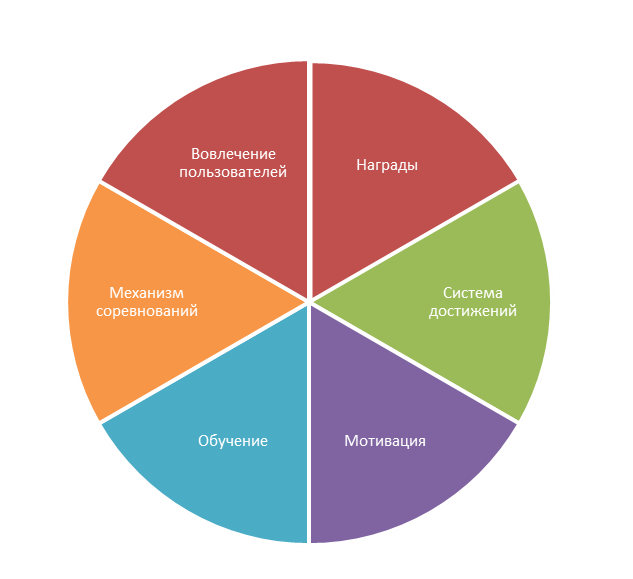
\includegraphics{flesh/gamification/gamification_pie.png}
	\caption{\label{fig:gamification_pie}Схема компонентов геймификации}
\end{figure}

Объединив приложение для тренировок с элементами игрового взаимодействия, можно ввести термин фитнес-игры. 

Фитнес-игра \textendash\space большой жанр игр, преимущественно для мобильных устройств, способствующих поддержанию здоровья игрока. Этот жанр позволяет игрокам геймифицировать свои тренировки: сделать процесс интереснее, веселее, увеличить мотивацию игрока к сохранению стабильной периодичности занятий.

Некоторые игры рассчитаны на одну конкретную активность, другие \textendash\space позволяют комбинировать разные их виды, тогда как третьи\,\textendash\space предлагают свои собственные виды активности для игрока.


Часто такого рода игры обладают минимально достаточным пользовательским интерфейсом:
\begin{itemize}
	\item Информация об активностях
	\item Интерфейс активной игровой сессии
	\item Окно статистики
\end{itemize}

Обычно игры этого жанра тесно интегрируются с устройствами отслеживания состояния игрока, включая, но не ограничиваясь данными с датчиков умных устройств:
\begin{itemize}
	\item Браслеты
	\item Часы
	\item Весы
	\item Смартфоны
	\item Наушники
	\item Умная обувь
\end{itemize}


В качестве примеров можно привести несколько известных игр такого жанра: 
\begin{description}
	\item[Zombies, Run! (2012)] Игра с глубоким погружением, геймифицирующая несколько видов бега и интервальных кардио тренировок. Сюжет разворачивается вокруг небольшого городка, являющегося большой базой выживших при зомби-апокалипсисе. Игрок бежит по открытой территории, собирает предметы в инвентарь, иногда убегает от зомби. Игра содержит несколько сезонов, представляющих из себя продолжения один другого и состоящих из миссий, каждая длинной от 30 до 60 минут.
	\item[Ingress (2013)] Многопользовательская игра с дополненной реальностью. Игра в стиле захвата флага, игроки поделены на две фракции. Потенциально геймифицирует пешие прогулки, не содержит сюжета, при этом позволяет игрокам ``захватывать порталы'' в реальном мире. Основная концепция \textendash\space возможность использовать ``таинственную энергию'' для связи порталов между собой, таким образом покрывая реальную карту многоугольниками с полем одной из двух фракций.
	\item[Pokémon Go (2016)] Многопользовательская игра с дополненной реальностью. Игра по мотивам одноименной серии аниме сериала, геймифицирующая пешие прогулки. Предлагает пользователям изучать местность, ловить покемонов и сражаться с игроками в реальном времени в публичных пространствах.
\end{description}

Все эти игры занимаются геймификацией разных видов активности. Игра, разрабатываемая в рамках данной работы будет геймифицировать один вид активности\,\textendash\space бег. 
